
\section{Introduction \& Motivation}\label{sect_intro}

The aim of this project is to identify popular topics over time, starting from tweets texts. Some key concepts for understanding the problem follow:
\begin{itemize}
  \item \textbf{Tweet}: a short text (sequence of words) sent at a specific time by a specific individual. The collection of terms that a tweet contains is collectively describing a message. The appearance of a term in many tweets makes the term popular.
  \item \textbf{Topic}: a set of terms. A popular topic is a set of terms that appear together in many tweets.
\end{itemize}

The goal of this work is not, however, to identify popular topics in a tweets dataset. The objective is to identify consistent topics in time, which means \textit{identifying set of terms that become frequent together throughout time}. The first step of the solution consists in identifying popular topics on every single day of the dataset. Then the results are merged to obtain all the itemset that are frequent in at least $n$ dates.

Solving the problem is very relevant because it not only allows researchers to investigate what are the causes that make a topic popular, but also to predict the reaction of the public in the future. Furthermore, the solution algorithm can be extended to solve many other similar problems where the initial premises are the same. The focus has been placed in the efficiency of the algorithm, so that it can be employed to solve similar problems with a large quantity of data, in a reasonable amount of time. Furthermore, importance was also given to the usability of the program.

%%%%%%%%%%%%%%%%%%%%%%%%%%%%%%%%

\section{Related work}\label{sect_rel_work}

The APriori algorithm is at the core of the solution algorithm presented in this report. In the proposed solution, there is an initial need to identify frequent, day-to-day sets of words. APriori is used in this operation. The results provided will then be combined in order to achieve the predicted objective: find frequent topics over time. APriori and its functioning will be briefly explained below, given their importance.

APriori is among the most used algorithms to solve the problem of finding frequent itemsets. Frequent itemsets are a form of frequent pattern. Given examples that are sets of items and a minimum frequency, any set of items that occurs at least in the minimum number of examples is a frequent itemset \cite{Toivonen2010}. In the specific case considered, the goal is to identify the words (items) that are frequently used in many tweets (set of items, or basket).

At the foundations of the APriori algorithm there is a simple, yet powerful, premise: a large set of items cannot be frequent unless all the subsets that compose it are frequent. Following the logic of this principle, the algorithm initially focuses on smaller sets. In such manner, it manages to eliminate large sets of items from the list of candidates. This is crucial for the optimization of the solution, since the algorithm does not have to try all the possible candidates.

%%%%%%%%%%%%%%%%%%%%%%%%%%%%%%%%

\section{Problem statement}\label{sect_probl_stat}

This section will specifically describe what input is required by the algorithm and what the generated output is.

\subsection*{Formal model}

\begin{itemize}
  \item $T =$ set of tweets, or sequences of words;
  \item $D =$ set of dates, one for each tweet.
\end{itemize}

It follows the utility function $u$.

$$ u: T \times D \rightarrow I \times D $$

where:
\begin{itemize}
  \item $I =$ set of topics (or itemset, group of words);
  \item Every topic of $I$ is present in a minimum of 2 dates.
\end{itemize}

\subsection*{Input}

The input required by the program is a dataset in \code{.pkl} format, necessary for the properties of the variables inside it to be maintained and recognized by the algorithm. There must be two columns in the dataset: \code{text} and \code{date}.

The \code{text} column contains texts of tweets. A tweet is defined as a sequence of words. For this reason, they are stored in the datasets as lists of words, or terms. Each term, or group of terms, is a potential frequent topic over time.

Every tweet must have an associated date. This is the purpose of the \code{date} column, which contains information regarding the day in which the tweet was posted, in the year-month-day format.

In order to fully understand the required input, it follows a small sample of the cleaned dataset used.

\begin{table}[h]
  \centering
  \begin{tabular}{@{}ll@{}}
  \toprule
  \textbf{date} & \textbf{text}                                         \\ \midrule
  2020-07-25    & {[}\textquotesingle smell\textquotesingle, \textquotesingle scent\textquotesingle, \textquotesingle hand\textquotesingle, \textquotesingle sanit\textquotesingle, \textquotesingle today\textquotesingle, ...{]} \\
  2020-08-29    & {[}\textquotesingle wear\textquotesingle, \textquotesingle cover\textquotesingle, \textquotesingle shop\textquotesingle, \textquotesingle includ\textquotesingle, \textquotesingle visit\textquotesingle, ...{]} \\
  ...           & ...                                                   \\ \bottomrule
  \end{tabular}
  \caption{Example of input data}
  \label{tab_input}
\end{table}

Notes: some words in Table \ref{tab_input} may appear truncated, other missing. It is intended, it will be explained in detail how the dataset was obtained in section \ref{sect_dataset}.

\subsection*{Output}

The interest is placed in finding groups of frequently repeated words within the tweets of several days, in order to find frequent topics over time. We assume that a group can also consist of a single word: even alone a word can identify a topic (for example \textit{mask}, or \textit{vaccine}).

Before proceeding with the output provided by the program, it is necessary to introduce the concept of \textbf{support}. It is a measure that allows to identify groups of frequent words based on a threshold value. The absolute support for an itemset $I$ is equal to the number of itemsets containing all items in $I$. Since there is a different number of tweets available for each day of the dataset, it is not feasible to use an absolute measure. For this reason it was used the relative support. In practice, the support was found by dividing the total number of times in which a group of words appeared in a day by the total tweets of that day. 

It is possible for the user to decide the \textit{support} value, when running the program. After numerous empirical tests, values around 0.015 are recommended. It is also possible to set the \textit{total number of results} to be obtained, as well as the \textit{minimum number of days} in which an itemset has to be present to be part of the final solution.

After running the algorithm, a dataset is obtained as an output. It has the following columns:

\begin{itemize}
  \item \code{itemsets}, groups of frequent words stored as a frozenset, representing the topics;
  \item \code{dates}, the list of days in which the itemset was frequent;
  \item \code{supports}, the list of the supports, one for each day in which the topic was frequent;
  \item \code{tot\_dates}, an absolute measure of the total days in which the itemset was found.
\end{itemize}

A sample of the output is provided in Table \ref{tab_output}.

\begin{table}[h]
  \centering
  \small
  \tabcolsep=0.14cm
  \begin{tabular}{@{}llll@{}}
  \toprule
  \textbf{itemsets}         & \textbf{dates}                     & \textbf{supports}      & \textbf{tot\_dates}  \\ \midrule
  (pandemic)                & {[}2020-7-24, 2020-7-25, ...{]}    & {[}0.03, 0.05, ...{]}  & 26                   \\
  (covid, trump)            & {[}2020-7-24, 2020-8-16, ...{]}    & {[}0.04, 0.07, ...{]}  & 24                   \\
  ...                       & ...                                & ...                    & ...                  \\
  (covid, india)          & {[}2020-7-25, 2020-7-26{]}           & {[}0.03, 0.04{]}       & 2                    \\ \bottomrule
  \end{tabular}
  \caption{Example of output data \label{tab_output}}
\end{table}

%%%%%%%%%%%%%%%%%%%%%%%%%%%%%%%%

\section{Solution}\label{sect_solution}

In this section, the solution will be explained in detail.

\begin{itemize}
  \item The first step is to divide the tweets according to their publication day (column \code{date} of the dataset).

  \item The APriori algorithm is then applied to each subgroup, consisting of all the tweets of a given day. In this way, frequent itemsets are obtained for each day of the dataset.
  
  \item Finally, the last part of the algorithm associates to each itemset found the dates in which it is frequent, together with their support.
\end{itemize}

It is possible to find all the aforementioned steps in Figure \ref{figSol}.

\begin{figure}[h]
  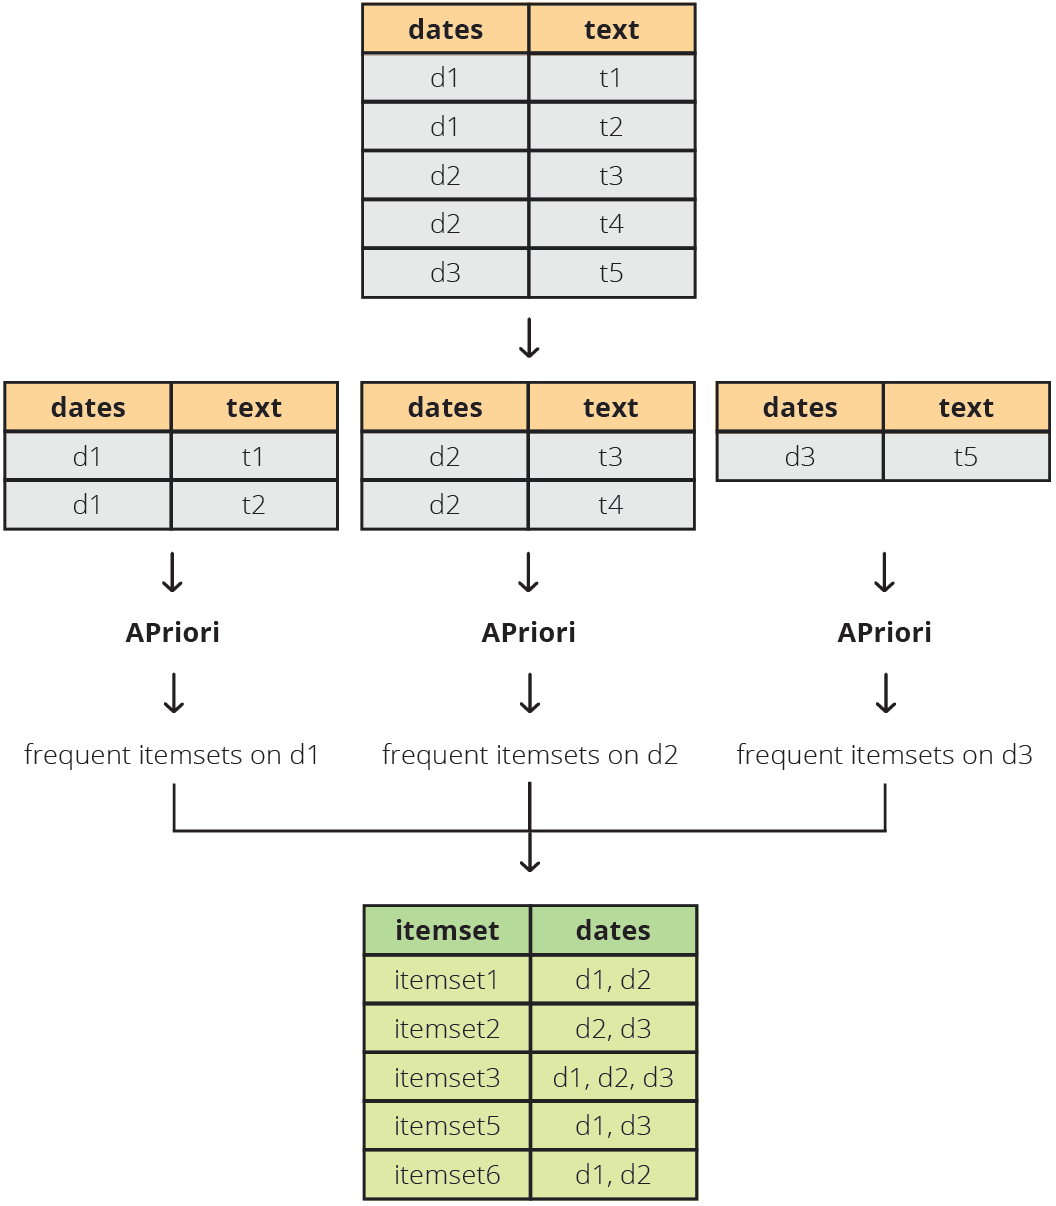
\includegraphics[scale=0.292]{solution.png}
  \centering
  \caption{graphical representation of the main steps of the algorithm}
  \label{figSol}
\end{figure} 

%%%%%%%%%%%%%%%%%%%%%%%%%%%%%%%%

\section{Implementation}\label{sect_impl}
It follows a description of the tools used to implement the solution reported in section \ref{sect_solution}.

\subsection*{Programming language}
To solve the problem, the Python language was used (version 3.8.5). It was chosen for its very simple syntax rules, which facilitate code readability and program scalability.

\subsection*{Libraries}
To work properly, the algorithm needs some libraries, some already present in Python, others that need to be installed. For each of them, a brief explanation follows.

\vspace{2mm}
\code{pandas} As described in the official website, pandas is a fast, powerful, flexible and easy to use open source data analysis and manipulation tool, built on top of the Python programming language \cite{pandas}. Moreover, it offers data structures and operations for manipulating numeric tables and time series.

\vspace{2mm}
\code{datetime} Built-in Python module that supplies classes for manipulating dates and times.

\vspace{2mm}
\code{time} Built-in Python module which provides various time-related functions. It is not strictly related to the algorithm, but is used to track the time taken by the program to solve the problem and notify the user.

\vspace{2mm}
\code{sys} Built-in Python module that provides access to some variables used or maintained by the interpreter and to functions that interact strongly with the interpreter. It has been used to manage the parameters specified by the user, in order to grant a solution suited to his needs.

\vspace{2mm}
\code{mlxtend} It is a library of Python tools and extensions for data science. Their implementation of the APriori algorithm was used in the final solution algorithm.

\vspace{4mm}
Note: detailed information about Python core packages can be found on their official website \cite{python_website}. 

%%%%%%%%%%%%%%%%%%%%%%%%%%%%%%%%

\section{Dataset}\label{sect_dataset}

\subsection*{Original dataset}

The original dataset is public, it was created by Gabriel Preda and can be found on the Kaggle website \cite{kaggle_df}.

The author specifies that the tweets were obtained through the use of the Twitter API and a Python script. All tweets contain the hashtag \#covid19, and cover a period of time from July 24, 2020 to August 30, 2020. However, in some days the tweets were not collected. In figure \ref{dates_and_tweets} it is possible to see how many tweets have been gathered for each day. 

\begin{figure}[h]
  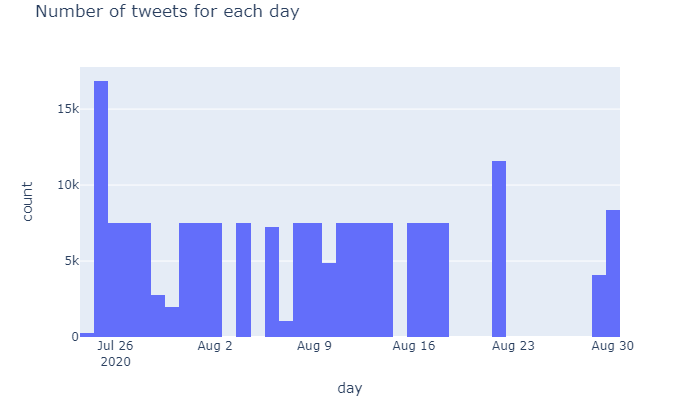
\includegraphics[scale=0.44]{dates_and_tweets.png}
  \centering
  \caption{number of tweets for each day}
  \label{dates_and_tweets}
\end{figure}

\subsection*{Column selection}

In addition to the texts of the tweets and the corresponding dates, the author has collected other variables, such as: 
\begin{itemize}
  \item \code{user\_location}
  \item \code{user\_name}
  \item \code{user\_description}
  \item \code{user\_created}
  \item \code{user\_followers}
  \item \code{user\_friends}
  \item \code{user\_favourites}
  \item \code{user\_verified}
  \item \code{source}
  \item \code{is\_retweet}
  \item \code{hashtags}
\end{itemize}

Since they are of no use to the study, they have been removed. As shown in section \ref{sect_probl_stat}, only the \code{text} and \code{date} columns have been preserved.

Column \code{date} originally contained information regarding the day and specific time the tweet was published. Only days were kept; information about the hours, minutes and seconds of the post were removed.

\subsection*{Text cleaning}

In the column \code{text}, the tweets texts are saved as a string. They are complete, therefore they contain punctuation, numbers, references to other users through the use of \code{@}, hashtags (and consequently the \code{\#} symbol), emojis, links, etc.

It is crucial to clean the texts so that they contain as much information as possible. To achieve this objective, various steps have been taken to obtain the final texts; they are reported below.

\subsubsection*{Lowercase text}
Each text was brought to its lowercase form, so that the algorithm does not differentiate words by capitalization.

\subsubsection*{Link removal}
Most tweets in the dataset are truncated. In these cases, the source link is shown at the end of the text, which adds no value to the tweet. Furthermore, users regularly post links that do not carry any semantic information. For this reason all links have been removed.

\subsubsection*{Punctuation, symbols and numbers removal}
Initially it was decided to keep the numbers, but various tests showed that not only did they not carry information, but segmented it. As for punctuation and symbols, it is clear that in this case they are not useful, and so they have been removed.

\subsubsection*{Stopwords removal}
Stopwords are extremely common words, like prepositions, conjunctions and some of the most common verbs. They carry little value to the meaning of the sentences. For this reason, each word is checked and if it is considered a stopword, it is removed from the sentence. There is no single stopwords dictionary, in the preprocessing the one provided by the \code{nltk.corpus} library was used.

\subsubsection*{Stemming}
Stemming is the process of reducing inflected or derived words to their word base form. It was used because, intuitively, similar words can refer to the same topic (e.g., scared, scary, scariest, etc.). An example of stemming can be seen in Figure \ref{stem}.

\begin{figure}[h]
  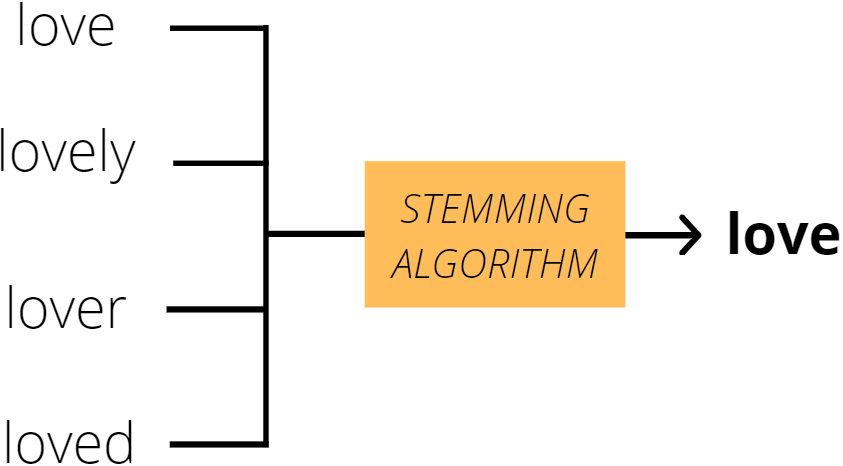
\includegraphics[scale=0.25]{stem.png}
  \centering
  \caption{simple example of stemming}
  \label{stem}
\end{figure}

\subsubsection*{From string to list of words}
It is easier and more intuitive to work with lists of terms, rather than with strings. So, list were chosen as the data type to store the tweets.

\vspace{4mm}
In order to clean all the texts, about 180,000 iterations had to be done. The process was quite time consuming: it took about 3 hours on an Intel Core i7-9700K processor. For this reason, the final clean dataset has been saved, ready to be used as an input to the algorithm.

%%%%%%%%%%%%%%%%%%%%%%%%%%%%%%%%

\section{Experimental Evaluation}\label{sect_exp_eval}

\textbf{Premise}: all tests reported in this section were carried out on the same machine, with the following components:
\begin{itemize}
  \item Intel Core i7-9700K processor
  \item DDR4-RAM 3600 MHz 2x8GB
  \item SSD NVMe PCIe M.2 2280 512Gb
  \begin{itemize}
    \item maximum read speed: 3400 megabyte/s
    \item maximum write speed: 3000 megabyte/s
  \end{itemize}
\end{itemize}

\subsection*{User evaluation}
In order to obtain a reasonable user evaluation, the algorithm code was sent to 10 people, along with instructions on how to execute it.

Five of these people are computer science graduates, thus they are accustomed to programming. None of them had problems running the code, despite using different operating systems (Windows, MacOS and Linux).

The other five are external to the world of information technology. Only one of them managed to successfully execute the code without external supervision. The problem others encountered was not with the instructions or execution of the specific code, but with the environment it requires to function properly. It was difficult for them to install the Python environment, manage environment variables and execute command line instructions. They needed outside supervision to be able to correctly run the code.

The best solution to make the code more accessible would be through the creation of an executable. Getting an executable from a \code{.py} Python script is not straightforward, but there are some libraries that make the process easier. It is possible to use the \code{pyinstaller} library, although there are some limitations. The first one is that the generated executable only works on the same type of operating system on which it was created. So, to cover most of the users, an executable for Windows, Linux and MacOS should be generated. Furthermore, in this specific case, the user still has to run the program from the command line, if he wants to use custom parameters. After giving the executable to the four people who had been having problems installing Python, they were able to successfully run the program.

A further improvement would consist in adding a graphical interface, with the possibility to choose the parameters to be used in the execution of the algorithm, as well as the possibility to select the initial dataset and where to save the final results.

\subsection*{Time comparison with baseline}

In the solution program, most of the computational cost lies in using the APriori algorithm to find itemsets that are frequent on each day of the dataset. Thus, the focus was mainly on its performance.

\subsubsection*{Naïve approach}
The problem of finding frequent itemsets can be approached naively. However, this entails enormous computational costs and limitations in the results obtained. Indeed, for a set of items $U$, there are a total of $2^{|U|}-1$ distinct subsets (if we do not consider empty subsets). The simplest way to get the results is to generate all these possible candidates and count how many times they appear in the dataset. It is intuitive to understand how, when $U$ is very large, this approach is impractical. As a simple example, just think that when $U = 1000$, there are $2^{1000}$ possible candidates, a number equal to about $10^{301}$. It is not possible for today's computers to keep all these information in the main memory.

\subsubsection*{APriori algorithm}
Given the impossibility of dealing with the problem in a naïve way, it was opted for the use of the APriori algorithm. The choice fell on this algorithm as it is well-established in the world of data mining, and for the completeness of the results it provides. As explained in section \ref{sect_rel_work}, APriori does not need to generate all possible candidates, which makes the algorithm much less computationally heavy. To justify the choice of using library \code{mlxtend}, a study was carried out on the resolution times of the first part of the final algorithm.

A baseline was selected: the implementation of APriori of the library \code{efficient-apriori }\cite{eff_apr}.

First it was made sure that the algorithms gave exactly the same results. Subsequently, each algorithm was run 100 times, with the following input:
\begin{itemize}
  \item the clean dataset, containing about 180,000 tweets, from a period from July 24, 2020 to August 30, 2020
  \item a support of 0.012
\end{itemize}

At the end of the execution, the average times of each algorithm were calculated. The results are reported in Table \ref{tab_apriori_times}.

\begin{table}[h]
  \centering
  \begin{tabular}{@{}lc@{}}
  \toprule
  \textbf{Library}     & \textbf{Average time (s)}                                         \\ \midrule
  mlxtend              & 20.7336 \\
  efficient-apriori    & 63.7155 \\ \bottomrule
  \end{tabular}
  \caption{Average execution time of \textit{mlxtend apriori} and \textit{efficient-apriori}}
  \label{tab_apriori_times}
\end{table}

It is clear from the results obtained that, although the output of the two algorithms is identical, the \code{mlxtend} version is much more optimized. On average, it takes a third of the time to perform the same calculations.


\subsection*{Scalability evaluation}
Finally, a test of the scalability of the program was performed. The APriori algorithm was run multiple times on a growing sample of tweets. Each run time was monitored. This simulates the time required to analyse a single day of the dataset. In Table \ref{tab_apriori_sc} and in Figure \ref{fig_times} it is possible to see how the times grow exponentially as the number of tweets increases. To compute the solution for a few thousand tweets the times vary from tenths of a second to a few seconds. However, when 256,000 tweets are considered, the time required to find the frequent itemset is about 34 minutes. Assuming an analysis is performed over 30 days, with 256,000 tweets for each day, the solution algorithm could take about $34 \cdot 30 = 1020$ minutes (about 17 hours) to deliver the results.  Considering the amount of data involved, it is not a poor result. During this last execution of the algorithm, all the RAM was being used. To further improve performance, it is possible to increase the available memory or rely on algorithms that, even if they not always provide complete results, are less computationally heavy. For this study it was preferred to have the certainty of obtaining complete results at the expense of some performance.

  
\begin{table}[h]
  \centering
  \begin{tabular}{@{}ll@{}}
  \toprule
  \textbf{N of tweets}   & \textbf{Time (s)}                                         \\ \midrule
  1,000                  & 0.043875 \\
  2,000                  & 0.141626 \\
  4,000                  & 1.259605 \\
  8,000                  & 2.731888 \\
  16,000                 & 1.588751 \\
  32,000                 & 3.834265 \\
  64,000                 & 14.126312 \\
  128,000                & 42.445597 \\
  256,000                & 2044.150201 \\ \bottomrule
  \end{tabular}
  \caption{Time of execution based on tweets number}
  \label{tab_apriori_sc}
\end{table}

\begin{figure}[h]
  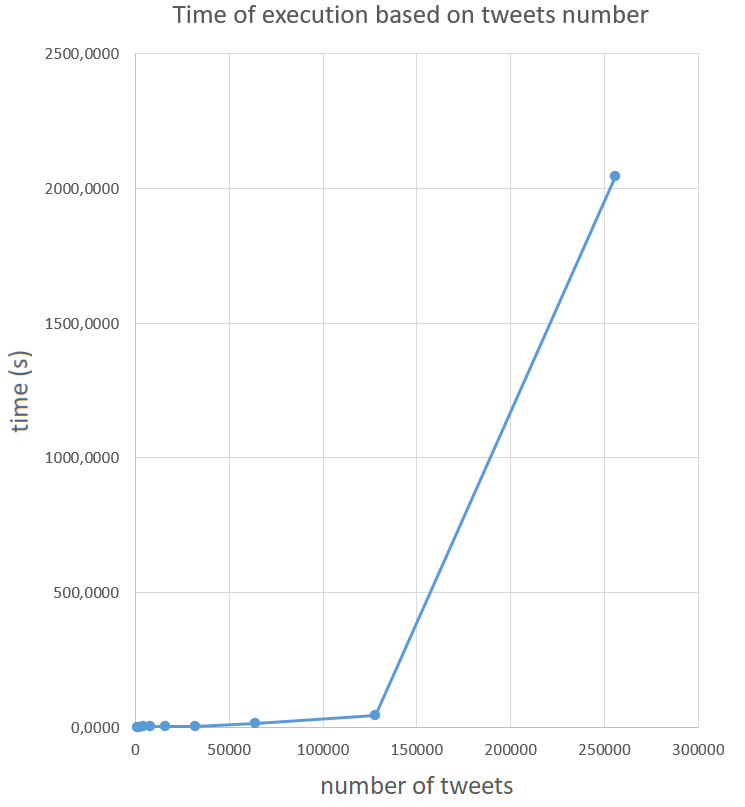
\includegraphics[scale=0.415]{scalability.png}
  \centering
  \caption{Time of execution based on tweets number}
  \label{fig_times}
\end{figure}

Note: the second part of the final solving algorithm is extremely fast and there are no substantial differences in terms of time, even with large datasets.

